% ======================================================================
% 7. přednáška – 14. 11. 2022
% Klasifikace elementárních částic (pokračování), kvantová čísla,
% kvarkový model, barva
% ======================================================================
\section{Klasifikace elementárních částic, kvantová čísla a kvarkový model}

\strana{P07-1}
\emph{7. přednáška, 14. listopadu 2022.}

\subsection{Klasifikace elementárních částic (pokračování)}

Na konci minulé přednášky jsme začali třídit „zoo“ částic, které experimenty
s kosmickým zářením a později na urychlovačích objevily. Takové třídění není
samoúčelné: pokud najdeme veličiny, které se v reakcích \emph{zachovávají},
můžeme předpovědět, které procesy jsou dovolené a které zakázané, a
z pravidelností v tabulce částic můžeme usuzovat na jejich vnitřní stavbu
(přesně tak, jako Mendělejevova tabulka vedla ke stavbě atomu). Částice lze
dělit podle spinu (fermiony vs.\ bosony) a podle toho, kterými interakcemi
působí (viz Davídkovy slajdy „Klasifikace částic, kvantová čísla“).

\begin{definice}[Hadrony a leptony]
\kw{Hadrony} jsou částice, které interagují silnou interakcí. Dělí se na
\begin{center}
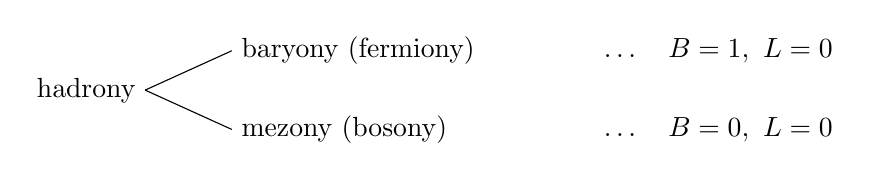
\begin{tikzpicture}[every node/.style={anchor=west}]
  \node (h) at (0,0) {hadrony};
  \node (b) at (2.6,0.5) {\kw{baryony} (fermiony)};
  \node (m) at (2.6,-0.5) {\kw{mezony} (bosony)};
  \draw (h.east) -- (b.west);
  \draw (h.east) -- (m.west);
  \node at (7.2,0.5) {\(\dots\quad B=1,\ L=0\)};
  \node at (7.2,-0.5) {\(\dots\quad B=0,\ L=0\)};
\end{tikzpicture}
\end{center}
\kw{Leptony} -- \(e,\ \mu,\ \nu_e,\ \nu_\mu,\ \dots\) -- jsou fermiony se
spinem \(S=\tfrac12\), nepodléhají silné interakci a mají \((B=0),\ L=1\).
\end{definice}

Zde \(B\) je \kw{baryonové číslo} a \(L\) \kw{leptonové číslo}. Obě jsou
\emph{aditivní} kvantová čísla: číslo systému je součtem čísel jednotlivých
částic, antičástice mají opačné znaménko. Dosud nebyl pozorován žádný proces,
který by \(B\) nebo \(L\) narušil -- odtud např.\ stabilita protonu (nejlehčí
baryon se nemá na co rozpadnout).

Ukazuje se, že leptonové číslo se zachovává dokonce \emph{zvlášť pro každou
rodinu} leptonů. Zavádíme proto elektronové a mionové leptonové číslo:
\[
  L_e(e)=1,\qquad L_\mu(\mu)=1 .
\]
Typickým příkladem je rozpad mionu
\[
  \mu^- \to e^- + \bar\nu_e + \nu_\mu .
\]
Zkontrolujme bilanci: vlevo \(L_\mu=1,\ L_e=0\); vpravo elektron dává
\(L_e=+1\), elektronové antineutrino \(L_e=-1\) a mionové neutrino
\(L_\mu=+1\). Obě čísla tedy souhlasí, a proto se v rozpadu musí objevit
\emph{dvě různá} neutrina. Kdyby se zachovávalo jen celkové \(L\), mohl by
probíhat i rozpad \(\mu\to e\gamma\), který ale nikdy pozorován nebyl.

\begin{vysvetleni}[Proč \(L_e\) a \(L_\mu\) zvlášť]
Neexistence rozpadu \(\mu\to e\gamma\) (experimentální limita větvicího
poměru je pod \(10^{-12}\)) je nejsilnějším argumentem pro oddělené
zachování \(L_e\) a \(L_\mu\). Dnes víme, že díky oscilacím neutrin se
rodinová leptonová čísla přesně nezachovávají (viz Davídkovy slajdy o
oscilacích neutrin), celkové \(L\) však ano.
\end{vysvetleni}

\subsection{Vlastnosti částic (kvantová čísla)}

Kromě aditivních kvantových čísel (\(Q,\ B,\ L\)) mají částice i
\kw{multiplikativní} kvantová čísla, která souvisejí s diskrétními
symetriemi -- zrcadlením prostoru (parita) a záměnou částice za antičástici
(nábojová parita).

\subsubsection*{Parita}
Operace parity \(\hat P\) převádí \(\vec r\to-\vec r\). Protože
\(\hat P^2=1\), jsou její vlastní čísla \(\pm1\). Celková parita stavu je
součinem \emph{vnitřních parit} částic a orbitální části \((-1)^{\ell}\).
Vnitřní paritu fermionů nelze absolutně změřit (fermiony vznikají vždy
v párech), proto se volí konvencí:
\[
  P(e^-)\equiv+1,\qquad P(p)\equiv P(n)\equiv+1 .
\]
Parity ostatních částic se pak určují z reakcí, které paritu zachovávají
(silná a elektromagnetická interakce). Pro piony vychází
\[
  P(\pi^+)=-1,\qquad P(\pi^0)=-1 ,
\]
piony jsou tedy \kw{pseudoskalární} částice (spin 0, záporná parita).
\pozn{u \(P(\pi^0)\) je znaménko minus v originále slabé, ale hodnota \(-1\) odpovídá skutečnosti}

\begin{vysvetleni}[Jak se měří parita pionu]
Klasicky z reakce \(\pi^- + d \to n + n\) se záchytem pomalého pionu ze stavu
\(s\) (\(\ell=0\)) pionového atomu. Ze zachování momentu hybnosti a
Pauliho principu pro dva neutrony vyplývá, že koncový stav je \(^3P_1\)
s paritou \(-1\); protože \(P(d)=+1\), musí být \(P(\pi^-)=-1\).
\end{vysvetleni}

\strana{P07-2}
\subsubsection*{\(C\)-parita (nábojová parita)}

Operátor nábojového sdružení \(\hat C\) zamění částici za její antičástici
(obrátí všechna aditivní kvantová čísla, ale ponechá hybnost a spin):
\[
  \hat C\ket{i}=\eta_c\ket{\bar i}, \qquad
  \hat C\hat C\ket{i}=\eta_c^2\ket{i} .
\]
Dvojí aplikace vrací původní stav, takže \(\eta_c^2=1\) a \(\eta_c=\pm1\).
Skutečným \emph{vlastním} stavem \(\hat C\) (s dobře definovanou
\(C\)-paritou) je ovšem jen částice, která je sama sobě antičásticí
(\(\gamma,\ \pi^0,\ \eta,\ \dots\)). Foton je kvantum elektromagnetického
pole, které při záměně nábojů mění znaménko, proto
\[
  C(\gamma)=-1 .
\]
Neutrální pion se rozpadá elektromagneticky na dva fotony, \(\pi^0\to2\gamma\).
Protože elektromagnetická interakce \(C\)-paritu zachovává a \(C\) je
multiplikativní,
\[
  C(\pi^0)=C^2(\gamma)=+1 .
\]
Odtud hned plyne předpověď: rozpad \(\pi^0\to3\gamma\) (s \(C=(-1)^3=-1\))
je zakázaný -- a skutečně nebyl pozorován.

\subsubsection*{Podivnost}

Koncem 40.\ a v 50.\ letech byly objeveny nové částice -- např.\
\(\Lambda^0\) a \(K\) -- s „podivným“ chováním:
\begin{itemize}
  \item vznikají v hojném počtu silnou interakcí, a to vždy \emph{v párech},
    např.
    \[ \pi^- + p \to \Lambda^0 + K^0 \qquad\text{(asociovaná produkce)}; \]
  \item \(\Lambda^0,\ K^0,\ \dots\) se ale rozpadají \emph{pomalu}
    (doby života \(\sim10^{-10}\,\mathrm{s}\), typické pro slabou interakci,
    zatímco silné procesy probíhají za \(\sim10^{-23}\,\mathrm{s}\)), a to
    více možnými kanály:
    \[
      \Lambda^0 \to p+\pi^-,\qquad \Lambda^0\to n+\pi^0, \qquad
      K^0\to\pi^0\pi^0,\quad \pi^+\pi^-\pi^0 .
    \]
\end{itemize}
Vysvětlení (Gell-Mann, Nishijima): zavedeme nové aditivní kvantové číslo
\kw{podivnost} \(S\), které silná a elektromagnetická interakce zachovávají,
ale slabá ne:
\[
  S(\Lambda^0)=-1,\qquad S(K^0)=+1 .
\]
V produkci \(\pi^-p\to\Lambda^0K^0\) je \(S\) vlevo i vpravo nulová, proto
jde silně. V rozpadu \(\Lambda^0\to p\pi^-\) se podivnost mění o jedničku,
což umí jen slabá interakce -- proto je rozpad pomalý.
\pozor{Pozor:} písmeno \(S\) zde označuje podivnost, nikoli spin.

\begin{definice}[Hypernáboj a izospin]
\kw{Hypernáboj} je definován jako
\[ \vzorec{Y\equiv B+S}. \]
Hadrony se stejným spinem, paritou a téměř stejnou hmotností (např.\ \(p\)
a \(n\)) tvoří \kw{izospinové multiplety}; jednotlivé členy rozlišuje třetí
komponenta izospinu \(I_3\). Náboj je pak dán
\kw{Gell-Mannovým--Nishijimovým vztahem}
\[ \vzorec{Q=I_3+\tfrac12\,Y}. \]
\end{definice}
Izospin vyjadřuje, že silná interakce „nevidí“ elektrický náboj -- proton a
neutron jsou pro ni dva stavy jedné částice (nukleonu) s \(I=\tfrac12\),
\(I_3=\pm\tfrac12\). Izospin zachovává jen silná interakce (viz tabulka
v Davídkových slajdech).

\subsection{Baryony a jejich multiplety}

\paragraph{Baryony se spinem \(\tfrac12\), \(P=+1\): \(J^P=\tfrac12^+\).}
Nejlehčí baryony jsou
\[
  p,\ n,\ \Lambda^0,\ \Sigma^+,\ \Sigma^-,\ \Sigma^0,\ \Xi^-,\ \Xi^0 .
\]
Vyneseme-li je do roviny \((I_3, Y)\), dostaneme pravidelný šestiúhelník se
dvěma částicemi ve středu -- \kw{baryonový oktet}:

\strana{P07-3}
\begin{center}
\begin{tikzpicture}[scale=1.5,
  bod/.style={circle,fill=ForestGreen,inner sep=1.6pt}]
  \draw[->] (-1.5,0) -- (1.6,0) node[right] {\(I_3\)};
  \draw[->] (0,-1.5) -- (0,1.5) node[above] {\(Y\)};
  \foreach \x/\l in {-1/-1,-0.5/-\frac12,0.5/\frac12,1/1}
    \draw (\x,0.05) -- (\x,-0.05) node[below=2pt] {\small\(\l\)};
  \draw (0.05,1) -- (-0.05,1) node[left] {\small\(1\)};
  \draw (0.05,-1) -- (-0.05,-1) node[left] {\small\(-1\)};
  \node[bod,label=above:{\(n\)}] at (-0.5,1) {};
  \node[bod,label=above:{\(p\)}] at (0.5,1) {};
  \node[bod,label=above:{\(\Sigma^-\)}] at (-1,0) {};
  \node[bod,label=above:{\(\Sigma^+\)}] at (1,0) {};
  \node[bod] at (0,0) {};
  \draw[ForestGreen] (0,0) circle (3.5pt);
  \node[ForestGreen] at (-0.22,0.2) {\small\(\Lambda^0\)};
  \node[ForestGreen] at (0.24,0.2) {\small\(\Sigma^0\)};
  \node[bod,label=below:{\(\Xi^-\)}] at (-0.5,-1) {};
  \node[bod,label=below:{\(\Xi^0\)}] at (0.5,-1) {};
\end{tikzpicture}
\end{center}
Každá vodorovná řada je izospinový multiplet: dublet nukleonů (\(Y=1\),
\(S=0\)), triplet \(\Sigma\) a singlet \(\Lambda\) (\(Y=0\), \(S=-1\)) a
dublet \(\Xi\) (\(Y=-1\), \(S=-2\)). Snadno ověříme vztah
\(Q=I_3+\tfrac12Y\), např.\ pro \(\Sigma^-\): \(-1+0=-1\), pro \(\Xi^0\):
\(\tfrac12-\tfrac12=0\).

\paragraph{Rozpady baryonů z oktetu.}
Všechny členy oktetu kromě protonu jsou nestabilní. Silně se rozpadat
nemohou -- nejlehčí stav s danou podivností nemá silný kanál -- a rozpadají
se tedy slabě (nebo elektromagneticky):
\[
  \Lambda^0:\ p\pi^-,\ n\pi^0; \qquad
  \Sigma\to\pi N,\quad \Sigma\not\to\pi\Lambda^0,\quad
  \Sigma^0\to\Lambda^0+\gamma; \qquad
  \Xi\to\pi\Lambda,\quad \Xi\not\to\pi\Sigma .
\]
Zakázané kanály jsou zakázány \emph{kinematicky}: \(m_\Sigma\approx
1190\,\mathrm{MeV}\) je menší než \(m_\Lambda+m_\pi\approx1116+135=
1251\,\mathrm{MeV}\), a podobně \(m_\Xi\approx1315\text{--}1322\,\mathrm{MeV}
< m_\Sigma+m_\pi\approx1324\,\mathrm{MeV}\). Neutrální \(\Sigma^0\) má
stejný kvarkový obsah jako \(\Lambda^0\) a je o \(77\,\mathrm{MeV}\) těžší,
proto přechází na \(\Lambda^0\) elektromagneticky vyzářením fotonu (bez
změny podivnosti, velmi rychle, \(\tau\sim10^{-19}\,\mathrm{s}\)).

\paragraph{Baryony se spinem \(\tfrac32\): \(J^P=\tfrac32^+\).}
Další skupinu tvoří těžší baryony -- \kw{rezonance} -- se spinem
\(\tfrac32\). V rovině \((I_3,Y)\) tvoří trojúhelník o deseti členech, tzv.\
\kw{dekuplet} (hmotnosti v MeV jsou v závorkách; členy jedné řady mají
přibližně stejnou hmotnost):
\begin{center}
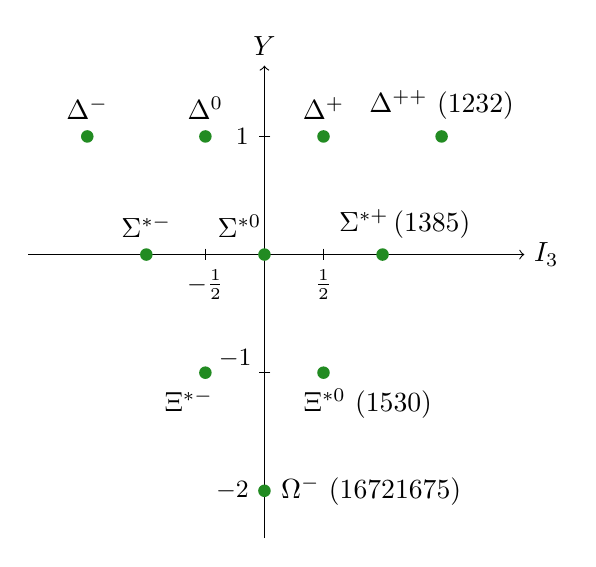
\begin{tikzpicture}[scale=1.5,
  bod/.style={circle,fill=ForestGreen,inner sep=1.6pt}]
  \draw[->] (-2,0) -- (2.2,0) node[right] {\(I_3\)};
  \draw[->] (0,-2.4) -- (0,1.6) node[above] {\(Y\)};
  \foreach \x/\l in {-1/-1,-0.5/-\frac12,0.5/\frac12,1/1}
    \draw (\x,0.05) -- (\x,-0.05);
  \node[below] at (-0.5,-0.05) {\small\(-\frac12\)};
  \node[below] at (0.5,-0.05) {\small\(\frac12\)};
  \draw (0.05,1) -- (-0.05,1) node[left] {\small\(1\)};
  \draw (0.05,-1) -- (-0.05,-1) node[left=-1pt,yshift=5pt] {\small\(-1\)};
  \draw (0.05,-2) -- (-0.05,-2) node[left] {\small\(-2\)};
  \node[bod,label=above:{\(\Delta^-\)}] at (-1.5,1) {};
  \node[bod,label=above:{\(\Delta^0\)}] at (-0.5,1) {};
  \node[bod,label=above:{\(\Delta^+\)}] at (0.5,1) {};
  \node[bod,label=above:{\(\Delta^{++}\ (1232)\)}] at (1.5,1) {};
  \node[bod,label=above:{\(\Sigma^{*-}\)}] at (-1,0) {};
  \node[bod,label={[xshift=-9pt]above:{\(\Sigma^{*0}\)}}] at (0,0) {};
  \node[bod,label={[xshift=8pt]above:{\(\Sigma^{*+}\,(1385)\)}}] at (1,0) {};
  \node[bod,label={[xshift=-6pt]below:{\(\Xi^{*-}\)}}] at (-0.5,-1) {};
  \node[bod,label={[xshift=16pt]below:{\(\Xi^{*0}\ (1530)\)}}] at (0.5,-1) {};
  \node[bod,label=right:{\(\Omega^-\ (\oprava{1672}{1675})\)}] at (0,-2) {};
\end{tikzpicture}
\end{center}
V poznámkách jsou \(\Sigma^*\) a \(\Xi^*\) psány jako \(\Sigma(\ )\),
\(\Xi(\ )\) -- prázdné závorky znamenají „stejná hmotnost jako vedlejší člen
řady“. Hvězdička odlišuje rezonance od stejnojmenných členů oktetu.

\begin{priklad}[Rozpady dekupletu]
\[
  \Delta\to\pi N, \qquad \Sigma^*(1385)\to\pi\Lambda, \qquad
  \Omega\not\to K\Xi .
\]
Rezonance \(\Delta\) a \(\Sigma^*\) mají dost hmotnosti na silný rozpad se
zachováním podivnosti (\(1232>938+140\), \(1385>1116+140\)), žijí proto jen
\(\sim10^{-23}\,\mathrm{s}\). Naproti tomu \(\Omega^-\) (podivnost \(-3\))
by se silně musel rozpadnout na \(K\Xi\) (\(S=-1-2=-3\)), ale
\(m_K+m_\Xi\approx494+1315=1809\,\mathrm{MeV}>m_\Omega\). Silný rozpad je
kinematicky zakázán, \(\Omega^-\) se rozpadá slabě (např.\
\(\Omega^-\to\Lambda K^-\)) a žije \(\approx10^{-10}\,\mathrm{s}\).
\end{priklad}

\begin{vysvetleni}[Předpověď \(\Omega^-\)]
V roce 1962 bylo známo jen devět členů dekupletu. Gell-Mann z pravidelnosti
hmotností (řady se liší zhruba o \(150\,\mathrm{MeV}\): \(1232,\ 1385,\
1530\)) předpověděl chybějící částici se \(S=-3\), \(Q=-1\) a hmotností
\(\approx1680\,\mathrm{MeV}\). Objev \(\Omega^-\) v Brookhavenu (1964)
s hmotností \(1672\,\mathrm{MeV}\) byl triumfem této klasifikace.
\end{vysvetleni}

\strana{P07-4}
Že jsou \(\Delta\) skutečně krátce žijící částice, vidíme na účinném
průřezu rozptylu pionů na protonech. Pro reakci
\[
  \pi^-+p\to\Delta^0\to\pi^0+n
\]
má závislost účinného průřezu \(\sigma\) na energii pionu \(E_\pi\)
výrazný \kw{rezonanční pík}:
\begin{center}
\begin{tikzpicture}[scale=1.1]
  \draw[->] (0,0) -- (5.5,0) node[below] {\(E_\pi\)};
  \draw[->] (0,0) -- (0,3.2) node[left] {\(\sigma\)};
  \draw[thick] (0.3,2.9) .. controls (0.9,1.7) and (1.4,0.9) .. (1.65,0.9)
    .. controls (1.8,0.9) and (1.8,2.6) .. (2.0,2.6)
    .. controls (2.3,2.6) and (2.5,0.9) .. (3.0,0.5)
    .. controls (3.5,0.25) and (4.5,0.15) .. (5.2,0.1);
\end{tikzpicture}
\end{center}
Šířka píku \(\Gamma\) souvisí s dobou života vztahem \(\tau=\hbar/\Gamma\);
pro \(\Delta\) je \(\Gamma\approx117\,\mathrm{MeV}\), tedy
\(\tau\approx6\cdot10^{-24}\,\mathrm{s}\) -- typická silná interakce.

\subsection{Kvarkový model}

\textbf{Jak to vysvětlit?} Pravidelné geometrické obrazce (oktety,
dekuplety) volají po vysvětlení podobně jako periodická tabulka. Odpovědí
je \kw{kvarkový model} (Gell-Mann, Zweig 1964): hadrony jsou složeny ze tří
druhů (vůní) kvarků \(d,\ u,\ s\), které samy tvoří v rovině \((I_3,Y)\)
trojúhelník:
\begin{center}
\begin{tikzpicture}[scale=1.8,
  bod/.style={circle,fill=ForestGreen,inner sep=1.6pt}]
  \draw[->] (-1,0) -- (1.2,0) node[below] {\(I_3\)};
  \draw[->] (0,-0.9) -- (0,0.9) node[above] {\(Y\)};
  \draw (-0.5,0.04) -- (-0.5,-0.04) node[below] {\small\(-\frac12\)};
  \draw (0.5,0.04) -- (0.5,-0.04) node[below] {\small\(\frac12\)};
  \draw (0.04,1/3) -- (-0.04,1/3) node[left] {\small\(\frac13\)};
  \node[left] at (0,-2/3) {\small\(-\frac23\)};
  \node[bod,label=above:{\(d\)}] at (-0.5,1/3) {};
  \node[bod,label=right:{\(u\)}] at (0.5,1/3) {};
  \node[bod,label=right:{\(s\)}] at (0,-2/3) {};
\end{tikzpicture}
\end{center}
Kvarky \(u,d\) tvoří izospinový dublet,
\[
  I(u,d)=\tfrac12:\qquad I_3(d)=-\tfrac12,\qquad I_3(u)=+\tfrac12,
\]
a protože baryon obsahuje tři kvarky, musí mít každý kvark
\[ B(u,d,s)=\tfrac13 . \]
Z Gell-Mannova--Nishijimova vztahu \(Q=I_3+\tfrac12Y\) pak plynou
\emph{zlomkové} náboje
\[
  Q(d)=-\tfrac13,\qquad Q(u)=+\tfrac23,\qquad Q(s)=-\tfrac13 .
\]
(Např.\ pro \(u\): \(Y=B+S=\tfrac13\), \(Q=\tfrac12+\tfrac16=\tfrac23\).)
Shrnutí kvantových čísel kvarků:
\strana{P07-5}
\begin{center}
\begin{tabular}{c|ccc}
  K.\,č. & \(u\) & \(d\) & \(s\)\\ \hline
  \(B\)   & \(\tfrac13\) & \(\tfrac13\) & \(\tfrac13\)\\[2pt]
  \(Q\)   & \(+\tfrac23\) & \(-\tfrac13\) & \(-\tfrac13\)\\[2pt]
  \(I_3\) & \(+\tfrac12\) & \(-\tfrac12\) & \(0\)\\[2pt]
  \(S\)   & \(0\) & \(0\) & \(-1\)
\end{tabular}
\end{center}
Antikvarky mají všechna tato čísla opačná. Všechny kvarky mají spin
\(\tfrac12\).

\subsubsection*{Baryony \((qqq)\)}
Složení baryonů z oktetu a dekupletu plyne prostým „sčítáním“ kvantových
čísel -- podivnost \(-1\) znamená jeden kvark \(s\), \(I_3\) určuje poměr
\(u\) a \(d\):
\[
\begin{aligned}
  p&=(uud), & n&=(udd), & \Lambda&=(uds), & \Sigma^-&=(dds),\\
  \Sigma^0&=(uds), & \Sigma^+&=(uus), & \Xi^-&=(dss), & \Xi^0&=(uss),
\end{aligned}
\qquad
\begin{aligned}
  \Delta^{++}&=(uuu),\\ \Omega^-&=(sss),\\ \Delta^-&=(ddd).
\end{aligned}
\]
Kontrola: \(Q(p)=\tfrac23+\tfrac23-\tfrac13=1\), \(Q(\Omega^-)=3\cdot(-\tfrac13)
=-1\). \(\Lambda\) a \(\Sigma^0\) mají stejný obsah \(uds\), liší se izospinem
dvojice \(ud\) (\(I=0\) vs.\ \(I=1\)). Ve spinu \(\tfrac12\) se tři kvarky
skládají tak, že dva spiny jsou antiparalelní; ve spinu \(\tfrac32\)
(dekuplet) jsou všechny tři paralelní.

\subsubsection*{Mezony \((q\bar q)\), \(J^P=0^-\)}
Mezony jsou vázané stavy kvarku a antikvarku. Antikvarky tvoří obrácený
trojúhelník (všechna kvantová čísla mají opačná):
\begin{center}
\begin{tikzpicture}[scale=1.6,
  bod/.style={circle,fill=ForestGreen,inner sep=1.6pt}]
  \begin{scope}
  \draw[->] (-0.9,0) -- (0.9,0) node[below] {\(I_3\)};
  \draw[->] (0,-0.9) -- (0,0.9) node[right] {\(Y\)};
  \node[bod,label=above:{\(d\)}] at (-0.5,1/3) {};
  \node[bod,label=above:{\(u\)}] at (0.5,1/3) {};
  \node[bod,label=right:{\(s\)}] at (0,-2/3) {};
  \node[ForestGreen] at (-1.1,0.9) {\(q\bar q\):};
  \end{scope}
  \draw[->,thick] (1.4,0) -- (1.9,0);
  \begin{scope}[xshift=3.3cm]
  \draw[->] (-0.9,0) -- (0.9,0) node[below] {\(I_3\)};
  \draw[->] (0,-0.9) -- (0,0.9) node[left] {\(Y\)};
  \node[bod,label=right:{\(\bar s\)}] at (0,2/3) {};
  \node[bod,label=below:{\(\bar u\)}] at (-0.5,-1/3) {};
  \node[bod,label=below:{\(\bar d\)}] at (0.5,-1/3) {};
  \end{scope}
\end{tikzpicture}
\end{center}
Pseudoskalární mezony (spiny \(q\) a \(\bar q\) antiparalelní, \(\ell=0\);
parita páru fermion--antifermion je \((-1)^{\ell+1}=-1\), odtud \(0^-\)):

\strana{P07-6}
\[
  \pi^+=(u\bar d),\quad \pi^-=(d\bar u),\qquad
  K^+=(u\bar s),\quad K^0=(d\bar s),\qquad
  \pi^0=\frac{1}{\sqrt2}\left(u\bar u-d\bar d\right).
\]
Neutrální pion je kvantově mechanickou superpozicí dvou stavů se stejnými
kvantovými čísly; znaménko minus odpovídá izospinu \(I=1\) (symetrická
kombinace by byla izospinový singlet). Podivnost \(K^+\) a \(K^0\) je
\(+1\), protože obsahují antikvark \(\bar s\) -- v souladu s \(S(K^0)=+1\)
z části o podivnosti.

\subsubsection*{Baryonový dekuplet v kvarkovém obsahu}
Dekuplet \(J^P=\tfrac32^+\) zapsaný pomocí kvarků:
\begin{center}
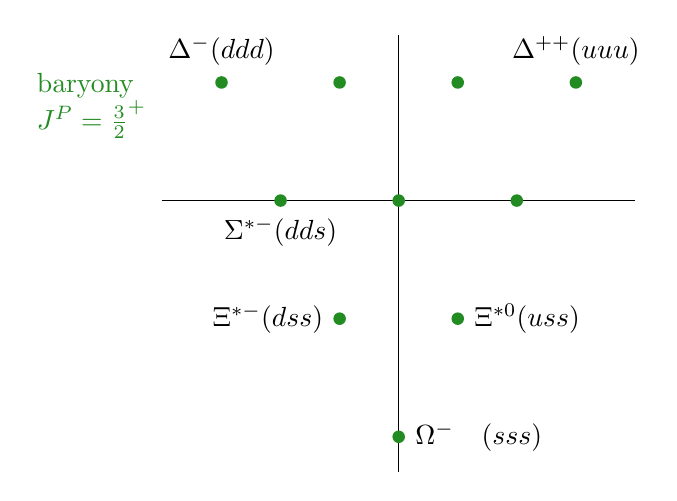
\begin{tikzpicture}[scale=1.5,
  bod/.style={circle,fill=ForestGreen,inner sep=1.6pt}]
  \draw (-2,0) -- (2,0);
  \draw (0,-2.3) -- (0,1.4);
  \node[bod,label=above:{\(\Delta^-(ddd)\)}] at (-1.5,1) {};
  \node[bod] at (-0.5,1) {};
  \node[bod] at (0.5,1) {};
  \node[bod,label=above:{\(\Delta^{++}(uuu)\)}] at (1.5,1) {};
  \node[bod,label=below:{\(\Sigma^{*-}(dds)\)}] at (-1,0) {};
  \node[bod] at (0,0) {};
  \node[bod] at (1,0) {};
  \node[bod,label=left:{\(\Xi^{*-}(dss)\)}] at (-0.5,-1) {};
  \node[bod,label=right:{\(\Xi^{*0}(uss)\)}] at (0.5,-1) {};
  \node[bod,label=right:{\(\Omega^-\quad(sss)\)}] at (0,-2) {};
  \node[ForestGreen,align=left] at (-2.6,0.8) {baryony\\ \(J^P=\frac32^+\)};
\end{tikzpicture}
\end{center}
Náboj \((dss)\) je \(-\tfrac13-\tfrac13-\tfrac13=-1\) a \((uss)\) je
\(\tfrac23-\tfrac23=0\); v poznámkách byly náboje \(\Xi^*\) posunuty o
jedničku: správně \(\oprava{\Xi^{*-}}{\Xi^0}=(dss)\) a
\(\oprava{\Xi^{*0}}{\Xi^+}=(uss)\).

\subsection{Barva a důkaz její existence}

Rohové stavy dekupletu \(\Delta^{++}=(uuu)\), \(\Delta^-=(ddd)\) a
\(\Omega^-=(sss)\) představují vážný problém: obsahují tři \emph{stejné}
fermiony ve stejném prostorovém stavu (\(\ell=0\), symetrický) se
symetrickou spinovou částí (všechny spiny paralelně, \(J=\tfrac32\)) a se
symetrickou vůňovou částí. Celá vlnová funkce by byla symetrická, což
odporuje \pozor{Pauliho principu}. Řešením je nové kvantové číslo
\kw{barva} se třemi hodnotami (červená, zelená, modrá); vlnová funkce je
v barvě antisymetrická a celek je pak antisymetrický. Hadrony jsou přitom
vždy „bezbarvé“ (barevné singlety). Teoretický argument je ale potřeba
potvrdit experimentem.

\begin{definice}[Poměr \(R\)]
\[
  R=\frac{\sigma(e^+e^-\to\text{hadrony})}{\sigma(e^+e^-\to\mu^+\mu^-)} .
\]
\end{definice}
Proč právě tento poměr? Oba procesy probíhají přes stejný mechanismus --
anihilaci \(e^+e^-\) na virtuální foton \(\gamma^*\), který se pak „rozpadne“
na pár nabitých fermionů:
\begin{center}
\begin{tikzpicture}[scale=1.1,
  fer/.style={thick,-{Stealth[length=5pt]}},
  fot/.style={thick,decorate,decoration={snake,amplitude=2.2pt,segment length=7pt}}]
  \begin{scope}
  \coordinate (v1) at (0,0); \coordinate (v2) at (2,0);
  \draw[fer] (-1.2,-1) -- (v1); \draw[fer] (v1) -- (-1.2,1);
  \node[left] at (-1.2,1) {\(e^+\)}; \node[left] at (-1.2,-1) {\(e^-\)};
  \draw[fot] (v1) -- (v2) node[midway,above=3pt] {\(\gamma^*\)};
  \draw[fer] (3.2,1) -- (v2); \draw[fer] (v2) -- (3.2,-1);
  \node[right] at (3.2,1) {\(\mu^+\)}; \node[right] at (3.2,-1) {\(\mu^-\)};
  \fill (v1) circle (2pt); \fill (v2) circle (2pt);
  \node[above right] at (v2) {\small\(Q(\mu)\)};
  \end{scope}
  \begin{scope}[xshift=6.5cm]
  \coordinate (v1) at (0,0); \coordinate (v2) at (2,0);
  \draw[fer] (-1.2,-1) -- (v1); \draw[fer] (v1) -- (-1.2,1);
  \node[left] at (-1.2,1) {\(e^+\)}; \node[left] at (-1.2,-1) {\(e^-\)};
  \draw[fot] (v1) -- (v2) node[midway,above=3pt] {\(\gamma^*\)};
  \draw[fer] (3.2,1) -- (v2); \draw[fer] (v2) -- (3.2,-1);
  \node[right] at (3.2,1) {\(q\)}; \node[right] at (3.2,-1) {\(\bar q\)};
  \fill (v1) circle (2pt); \fill (v2) circle (2pt);
  \node[above right] at (v2) {\small\(Q(q)\)};
  \end{scope}
\end{tikzpicture}
\end{center}
Šipky na fermionových liniích ukazují tok fermionového čísla (antičástice
jde „proti šipce“). Amplituda je úměrná náboji ve vrcholu, kde vzniká
koncový pár, účinný průřez tedy jeho kvadrátu. Vše ostatní (elektronový
vrchol, propagátor fotonu, kinematika při energiích daleko nad prahem) se
v poměru vykrátí. Vzniklý pár \(q\bar q\) se pak s pravděpodobností 1
přemění na hadrony (hadronizace). Proto
\[
  R=N_c\sum_q Q_q^2 ,
\]
kde \(N_c\) je počet barev -- každý barevný stav kvarku je samostatný
koncový stav a jejich příspěvky se sčítají. Pro energie, kde lze vytvořit
jen \(u,d,s\) (\(\sqrt s\lesssim3\,\mathrm{GeV}\)):

\strana{P07-7}
\[
  R=3\times\frac{\left(\frac23\right)^2+\left(-\frac13\right)^2+
  \left(-\frac13\right)^2}{1}=3\times\frac23=\vzorec{2}
\]
(ve jmenovateli je \(Q(\mu)^2=1\)). Bez barvy bychom čekali
\(R=\tfrac23\); měření dávají \(R\approx2\), což je přímý experimentální
důkaz, že kvarky existují ve \emph{třech} barvách.

\begin{vysvetleni}[Průběh \(R\) s energií]
Nad prahem tvorby párů \(c\bar c\) (\(\sqrt s\approx3{,}7\,\mathrm{GeV}\))
přibude člen \(3\cdot(\tfrac23)^2=\tfrac43\), takže \(R\to\tfrac{10}3\); nad
prahem \(b\bar b\) pak \(R\to\tfrac{11}3\). Tyto schody jsou v datech
skutečně vidět, i když je zakrývají ostré píky rezonancí
(\(J/\psi,\ \Upsilon,\dots\)) a logaritmická škála (viz Davídkovy slajdy
„Existence barvy“).
\end{vysvetleni}
